\documentclass[12pt,a4paper,norsk]{article}
\usepackage[utf8]{inputenc}
\usepackage[norsk]{babel}
\usepackage{hyperref} % for hyperlenker mellom ref og label
\usepackage{amsmath}
\usepackage{amssymb}
\usepackage{amstext} % for \text macro
\usepackage{array}   % for \newcolumntype macro
\newcolumntype{C}{>{$}c<{$}} % math-mode version of "l" column type
\usepackage{siunitx}
\usepackage{subcaption} %for subfigure
\usepackage{float}
\usepackage{booktabs} %for nice table lines
\usepackage[siunitx, american, europeanresistors, RPvoltages]{circuitikz} % for kretser
\usepackage{graphicx} % for bilder
\graphicspath{{./}}

\usepackage[skip=5mm]{parskip} % mellom mellom paragrafer, ikke indent
\usepackage{caption} % For å putte caption på figurer i minipage
\usepackage{xcolor} % Farger :)
\usepackage{tikz-timing} % For rising og falling edge

\newcommand{\resi}[1]{\frac{1}{#1}}
\newcommand{\red}[1]{{\color{red}#1}}
\newcommand{\rising}{\texttiming{[-,timing/slope=0]LH}}
\newcommand{\falling}{\texttiming{[-,timing/slope=0]HL}}

\title{Krets og digitalteknikk}
\author{Håvard Krogstie}
\date{\today}

\begin{document}

\maketitle

\noindent
Dette dokumentet inneholder definisjoner og formler brukt i krets- og
digitalteknikk. I tillegg forklares en del metoder. Dette er på ingen måte en
lærebok, men kan brukes til oppslag og oppfriskning. Ting kommer i en grei
rekkefølge, men noen formler og regler brukes før de defineres. Dokumentet har
ikke figurer for alt, så det er greit å ha et indre bilde av kretser. I
kretsdelen står blant annet grunnleggende kretsteori, metoder for regning på
kretser og formler for kondensatorer og spoler. I digitalteknikkdelen kommer
dioder og transistorer, CMOS, logiske kretser, boolsk algebra,
binærtallsregning, timing av digitale kretser og sekvensielle kretser.

\tableofcontents
\clearpage

\section{Kretser}
Kretser er samlinger med komponenter koblet sammen. Kretsen kan modeleres som en
graf der koblinger er noder. Komponentene blir kanter mellom
nodene. Ofte ser vi ikke på ledninger som komponenter, men bare som
ideelle koblinger. Noder med kun ledninger i mellom blir dermed samme node. Det
går strøm mellom nodene gjennom komponentene som binder dem sammen. Nodene har
også en egenskap kalt potensiale. Vi har lover for å regne på disse.

\subsection{Strøm og ladning}
Ladning er en elektromagnetisk egenskap ved blant annet elektroner. Den måles i
Coulomb (\si{\coulomb}). Strøm betyr flyt av ladning over tid, og måles i ampere
(\si{\ampere}) etter formelen
\[\SI{1}{\ampere} = \SI{1}{\coulomb\per\second}\]
Strøm går altså gjennom en ledning eller et komponent, og kan måles ved å
erstatte ledningen med et amperemeter. Vi kaller ofte strøm for $I$ eller $i$.

\subsection{Spenning}
Spenning er en differanse i potensiale mellom to noder i en krets. Spenning
måles i Volt (\si{\volt}), og er energi per ladning (\si{\joule\per\coulomb}).
Spenning må altså alltid ses som en potensialforskjell mellom to steder i en
krets, så det er ikke egentlig mulig å ha spenning i et bestemt punkt, med
mindre et annet punkt er definert til å være nullpunktet, jord (GND). Vi kaller
ofte spenning for $V$ eller $v$. Andre bruker $U$ for spenning.

\subsection{Effekt}
Observer at
\[\SI{1}{\volt} \cdot \SI{1}{\ampere} = \SI{1}{\joule\per\coulomb} \cdot \SI{1}{\coulomb\per\second} = \SI{1}{\joule\per\second} = \SI{1}{\watt}\]
Dette gir oss formelen for effekt i et komponent.
\[P = V \cdot I\]

\subsection{Kirchoffs strømlov}
Kirchoffs strømlov (KCL) sier at
summen av strømmer inn i en node er alltid lik 0. Hvis det kommer
\SI{5}{\ampere} inn i en node, må det altså gå \SI{5}{\ampere} ut igjen òg. En
node kan ha vilkårlig mange kanter ut av seg, og en denne definisjonen på node
kan også inneholde komponenter. Det viktige er at du teller alle ledninger som
går inn og ut av noden.

Et resultat av KCL er at det ikke kan gå strøm i en åpen krets, altså en ledning
som bare er koblet til noe i éne enden.

\subsection{Kirchoffs Spenningslov}
Kirchoffs spenningslov (KVL) sier at summen av spenningsfallet over enhver løkke må
være lik 0. Spenningsfall over et komponent er potensialforskjellen mellom
nodene den er koblet til. En løkke er en sti gjennom kretsen som stopper der den
starter, og KVL sikrer at potensialet til startnoden og stoppnoden er det
samme, hvilket det burde være siden de er samme node.

\subsection{Passiv fortegnskonvensjon}
Når man skal sette hvilken vei spenningen går over et komponent, setter man den
slik at $P = V \cdot I$ er positiv for laster, og negativ der det tilføres
energi til kretsen. Effekt inn må være lik effekt ut (Det må ikke nødvendigvis
skje samtidig, f.eks.\ om noe energi lagres i en kondensator).
Resultatet for dette er at vi anser \textit{spenningsfallet} over en last som
positivt, og over en spenningskilde som negativt.

NB!\@ Det er mulig for en spenningskilde å ha positivt spenningsfall, dersom
strømretningen går fra $+$ til $-$. En motstand har \textbf{alltid} positivt
spenningsfall.

\section{Kilder}
Det kan være mange komponenter som tilfører strøm eller spenning. Vi ser på 4
idealiserte utgaver. Uavhengige strøm- og spenningskilder leverer henholdsvis
strøm og spenning. Uansett hva som skjer ellers i kretsen garanterer kildene en
viss strøm gjennom en ledning, eller en viss potensialforskjell mellom noder.
Avhengige kilder gir samme garanti, men hvilken strøm/spenning som leveres er
avhengig av noe. For eksempel kan en spenningskilde levere 5 ganger
spenningsfallet over en gitt motstand.

På grunn av lovene vil det gå ofte gå strøm gjennom en spenningskilde, og en strømkilde
kan ha spenningsfall. På grunn av den passive fortegnskonvensjonen
vil ofte spenningskilder ha negativt spenningsfall, men det er ikke sikkert. F.
eks.\ i serie med en motsatt rettet sterkere spenningskilde.

Det finnes også AC-kilder som leverer vekselstrøm med oppgitte frekvenser og bølgeformer.

\subsection{Nulle ut}
Man kan ønske å nulle ut en kilde slik at den ikke bidrar (f.eks.\ i
superposisjon). En spenningskilde blir en kortslutning for å garantere $V=0$,
mens en strømkilde blir en åpen krets for å garantere $i=0$.

\section{Motstand}
Motstand er en egenskap ved komponenter som begrenser flyten av strøm. Forholdet
mellom strøm ($I$), spenning ($V$) og motstand ($R$) er gitt ved Ohms lov.
\[V = R \cdot I\]
Motstanden måles i \si{\ohm}. En ideell motstand har samme $R$ for alle $I$. Når
vi bruker komponentet vi kaller motsand, regner vi med at den er ideell. $I(V)$
er da en proposjonal funksjon, og grafen er en linje. Andre komponenter, slik
som lysdioder, har helt andre grafer for $I(V)$-funksjonen.

\subsection{Effekt}
Ohms lov kombineres med formelen for effekt.
\[P = V \cdot I = RI^{2} = \frac{V^{2}}{R}\]
Disse formlene gjelder i enhver last. I en vanlig motstand blir effekten om til
varmeenergi.

\subsection{Seriekobling}
Seriekoblede mostander oppfører seg som én motstand $R_{eq}$ der
\[R_{eq} = R_{1} + R_{2}\]

\subsection{Parallellkobling}
Parallellkoblede motstander må hva samme spenningsfall over hver motstand, men
strømmen blir forskjellig. To parallellkoblede motstander $R_{1}$ og $R_{2}$ vil
oppføre seg identisk med én motstand $R_{eq}$ der
\begin{align*}
  \resi{R_{eq}} &= \resi{R_{1}} + \resi{R_{2}} \\
  R_{eq} &= \resi{\resi{R_{1}} + \resi{R_{2}}} \\
        &= \frac{R_{1}R_{2}}{R_{1} + R_{2}}
\end{align*}
Strømmen får flere veier å gå, så $R_{eq}$ er mindre enn både $R_{1}$ og $R_{2}$.

\section{Nodespenningsmetoden}
Se på potensialet i vesentlige noder i forhold til en nullspenning (jord). Bruk Ohms
lov og spenningsdifferansen mellom noder $v_{\_}-v_{\_}$ for å regne
$i_{\_} = \frac{v_{\_}-v_{\_}}{R_{\_}}$. Sett deretter uttrykkene for strøm gitt
nodespenning inn i \textit{KCL} for hver node for å få et ligsningssett med
nodespenninger.

\section{Superposisjon}
TODO\@: Skriv

\section{Thévenin-ekvivalenten}
Enhver lineær krets med kun kilder og motstander vil sett fra to terminaler
kunne erstattes med en enkel krets med kun en spenningskilde $V_{Th}$ og en
motstand $R_{Th}$.
Vi kan finne $V_{Th}$ ved å se på spenningen over den åpne kretsen mellom
terminalene i den opprinnelige kretsen.
Vi kan finne $R_{Th}$ ved å nulle ut alle kilder og måle $R_{eq}$ over
terminalene. Vi kan også regne ut $R_{Th}$ ved å se på strømmen over terminalene
ved kortslutning: $R_{Th} = \frac{V_{Th}}{I_{SC}}$

\section{Kondensatorer}
Kondensatorer består av to ledende plater (elektroder) separert av en isolator,
ofte laget av et dielektrisk element. Kapasitansen $C$ måles i farad
(\si{\farad}) og er gitt ved arealet til platene $A$, avstanden mellom platene
$d$, og isolatorens permittivitet $\epsilon$.
\[C = \frac{A \epsilon}{d}\]
Det går ikke strøm mellom platene, men platene kan lades opp med en
spenningsforskjell $v$. Da får platene en ladning på $+Q$ og $-Q$, gitt ved
\[Q = C \cdot v\]
Dette gir oss at \SI{1}{\farad} = \SI{1}{\coulomb\per\volt}. Dette er svært mye,
så kondensatorer opererer gjerne med \si{\micro\farad}.
Den deriverte av ladning med hensyn på tid $\frac{dQ}{dt} = i(t)$, så vi får
formelen
\[i(t) = C \cdot \frac{dv}{dt}\]
Dette betyr at strømmen er proposjonal med forandring i spenning. I en krets
vil ikke spenningen over en kondensator kunne endres momentant, siden det ville
gitt uendelig høy strøm. Spenningen endrer seg gradvis, og når den har nådd
målspenningen vil $i(t) = 0$. Dette kalles \textit{steady state}.

\subsection{Regning på kondensatorer}
I en krets vil platene i en kondensator alltid være motsatt ladet, altså $+Q$ og $-Q$.
Selv om kondensatoren ikke lar strøm passere, så vil det derfor likevel virke
slik når den lades opp eller ut. Kirchovs strømlov gjelder fortsatt, så man kan
ikke tilføre strøm til én plate uten at det kommer like mye strøm ut fra den andre
platen. Dette høres kanskje trivielt ut, men det er lett å tro at strømmen
mellom to kondensatorer lever sitt eget liv, og at ladning kan bevege seg fritt mellom
platene på innsiden. Figur~\ref{fig:capacitor_Q} viser at $i(t)$ oppfører seg helt
vanlig sett utenifra.
%
\begin{figure}[H]
  \centering
  \begin{circuitikz} \draw
    (0,0) to[V]
    (0,4) to[R=$R$, i=$i(t)$] (4,4)
    to[C=$C_{1}$] (4,2.5)
    to[short, i=$i(t)$] (4,1.5)
    to[C=$C_{2}$] (4,0)
    to[short, i=$i(t)$] (2.5,0) to[short, o-o] (1.5,0) -- (0,0);
  \end{circuitikz}
  \caption{Kirchovs strømlov gjelder fortsatt for kondensatorer \label{fig:capacitor_Q}}
\end{figure}
%
\noindent
I en AC-krets vil det se ut som strøm passerer gjennom kondensatoren.

\subsection{Eksempler på kondensatorer}
Én type er små gule/brune kjeramiske kondensatorer. De har ikke polaritet. Det
finnes også sylinderformede elektrolyttkondensatorer som har polaritet. I
tillegg er det verdt å merke seg at alle ledninger med isolasjon mellom seg vil
ha en viss kapasitans. Dette betyr at nærhet mellom ledninger kan påvirke hvor
raskt signaler (spenning) i ledningene klarer å endre seg. En ledning med kontinuerlig
strøm vil også indusere et magnetfelt rundt seg, se seksjon~\ref{sec:spoler} om
spoler.

\subsection{Eksempelbruk av kondensator}
Kapasitans kan tenkes på som en treghet i spenning. Et eksempel på bruk er
mellom VDD og jord på en chip. Se figur~\ref{fig:capacitor_VDD}. Chippen kan gjøre
mye forskjellig, og mengden strøm som brukes kan variere. Når strømforbruket $i$
øker vil spenningsfallet over $R$ øke, men chippen har lyst på så jevn spenning
som mulig. Derfor har vi en kondensator som motvirker forandring i $V$.
Kondensatoren tilfører ekstra strøm $i_{C}$ når chippen trenger det, slik at $i$
blir så jevn som mulig. Spenningsfallet over $R$ blir dermed mer stabilt. Når
chippen bruker mindre strøm vil kondensatoren ta til seg strøm for å holde $i$
stabil.
%
\begin{figure}[H]
  \centering
  \begin{circuitikz} \draw
    (0,0) to[V]
    (0,4) to[R=$R$, i=$i$]
    (6,4) -- (8,4) -- (8,3.5) node[below]{VDD}
    -- (7,3.5) -- (7,.5) -- (8,.5) node[above]{GND}
    -- (8,0) -- (0,0)
    (6,0) to[C, i=$i_{C}$, *-*] (6,4)
    (8,3.5) -- (10,3.5) -- (10,.5) -- (8,.5)
    (5.5,4) to[open, v=$V$] (5.5,0);
  \end{circuitikz}
  \caption{Kondensator som spenningsstabisator\label{fig:capacitor_VDD}}
\end{figure}
%
\noindent
Kondensatoren tar på ingen måte bevisste valg om å gi og ta strøm. Det er et
resultat av at spenningsfallet over kondensatoren er proposjonalt med ladningen
den har. For å endre spenning må den strømme inn eller ut ladning.
Kondensatoren ``prøver'' altså å tilpasse seg forandringer i spenningen rundt,
men må først kvitte seg med ladning. Denne strømmen motvirker forandringene, men
kondensatoren lades samtidig opp eller ut. Dersom chippen over tid bruker mer
strøm, vil spenningen over kondensatoren etterhvert stabiliere seg ved den nye
standaren. Kondensatoren motvirker altså raske forandringer, men er ikke en
spenningsregulator.

\subsection{Energi}
Mengden energi i en kondensator regnes med formelen
\[E_{C} = \resi{2} C v^{2}\]

\subsection{Seriekobling}
Seriekoblede kondensatorer får avstanden mellom platene summert, så kapasitansen
blir lavere. Spenningsfallet over hver kondensator blir også lavere.
\[C_{eq} = \resi{\resi{C_{1}}+\resi{C_{2}}}\]

\subsection{Parallellkobling}
Parallellkobling av kondensatorer gir mer plate å lade. Kapasitansen blir større.
\[C_{eq} = C_{1} + C_{2}\]

\section{Spoler}\label{sec:spoler}
TODO\@: Skriv
\subsection{Seriekobling}
TODO\@: Skriv
\subsection{Parallellkobling}
TODO\@: Skriv

\section{RC-krets}
$\tau = RC$

\section{RL-krets}
$\tau = \frac{L}{R}$

\clearpage
\addcontentsline{toc}{section}{Digitalteknikk}
\begin{center}
  {\LARGE Digitalteknikk}
\end{center}

\section{Dioder}\label{sec:dioder}
TODO\@:Skrive om doping, hull og spenningsbarriærer.

\section{Transistorer}
Transistorer er komponenter som bruker en strøm eller spenning til å regulere
flyten av strøm eller spenning. De kan brukes både som forsterkere og brytere.

\subsection{MOSFET}
MOSFET (Metal-oxide-semiconductor field-effect transistor) er en type
transistor som bruker dopede halvledere for å kontrollere strøm. Se
seksjon~\ref{sec:dioder} om dioder. MOSFET tegnes ofte som et vindu med
gardiner, der vinduet er p/n-dopet, og gardinene er motsatt n/p-dopet. Det er
dopingen på gardinene som bestemmer om det er pMOS eller nMOS. Se figur~\ref{fig:nMOS}.

\begin{figure}[hbt!]
  \centering
  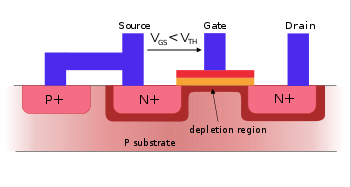
\includegraphics[width=0.6\textwidth,height=\textheight,keepaspectratio]{Krets_nMOS}
  \caption{Tverrsnitt av nMOS fra Wikipedia\label{fig:nMOS}}
\end{figure}

Til den éne gardinen kobles terminalen \textit{source} (S). Til den andre
gardinen \textit{drain} (D). Strøm klarer ikke å passere mellom dem til vanlig,
siden man får spenningsbarriærer mellom viduet og gardiene. En tredje terminal,
\textit{gate} (G) er koblet til en \textbf{metall}plate med et isolerende
\textbf{oksid}lag, som ``kobler'' source og drain. Gate er isolert, så det går
ikke faktisk strøm, men platen kan lades opp likt en kondensator, der vinduet er
den andre platen. Viduet må da være koblet opp til en fjerde terminal,
\textit{body} (B), slik at gate har en spenning å være relativ til. Når gate og
body har en spenningsforskjell riktig vei over terskelspenningen $V_{TH}$,
dannes en bru av positiv eller negativ ladning mellom gardinene. Avhengig av
dopingen lar én av disse strøm passere mellom source og drain.
%
Ofte har transistorer bare tre terminaler. Det er fordi body kobles opp til
source. Da måles gatespenning $V_{GS}$ relativt til sourcespenning $V_{S}$: \\
%
pMOS lukkes mellom \textit{source} og \textit{drain} når $V_{GS} \ll V_{S}$\\
nMOS lukkes mellom \textit{source} og \textit{drain} når $V_{GS} \gg V_{S}$\\
Her betyr $\ll$ en differanse på mer enn terskelspenningen $V_{TH}$. Eksempel på
terskelspenning: \SI{0.45}{\volt}.

\subsection{CMOS}\label{sec:cmos}
CMOS (Complementary Metal-oxide-semiconductor) er et system for design av
logiske kretser med MOSFET\@. Det baserer seg på symmetriske par av pMOS
og nMOS koblet opp til $V_{DD}$, $V_{SS}$, inputs og hverandre.
$V_{DD}$ er drain, og er høy (f.eks. \SI{5}{\volt}). $V_{SS}$ er source, som er
lav, altså jord.
%
\begin{figure}[hbt!]
    \centering
    \begin{circuitikz} \draw
    (0,1) node[pmos](ap){}
    (2,1) node[pmos](bp){}
    (1,-1) node[nmos](an){}
    (1,-2) node[nmos](bn){}

    (ap.S) -- ++(1,0) -- ++(0,.3) node[odiamondpole]{$V_{DD}$}
    (bp.S) -- ++(-1,0)

    (ap.G) node[left]{A}
    (bp.G) node[left]{B}
    (an.G) node[left]{A}
    (bn.G) node[left]{B}

    (bn.S) node[ground]{} node[below right]{$V_{SS}$}

    (ap.D) -- (0, 0) -- (4,0) node[odiamondpole]{Out}
    (bp.D) to[short,-*] (2,0)
    (an.D) to[short,-*] (1,0)
    ;
    \end{circuitikz}
    \caption{En NAND-port i CMOS \label{fig:CMOS_NAND}}
\end{figure}

%
CMOS følger regler for oppsett. En \textbf{pMOS} sin \textit{source} er alltid
koblet til $V_{DD}$ eller til en annen pMOS sin \textit{drain}. En \textbf{nMOS}
sin \textit{source} er alltid koblet til $V_{SS}$ eller til en annen nMOS sin
\textit{drain}\@. pMOS brukes altså til opptrekk av output, og nMOS brukes til
nedtrekk av output. \textit{Complementary} betyr at kun én av trekkene på output
kan være lukket. Se figur~\ref{fig:CMOS_NAND}.
%
\subsubsection{Viktig å huske om CMOS}
\begin{itemize}
  \item CMOS bruker kun strøm på å endre ladning i gate i MOSFETene. Det betyr at det
    kun går strøm til input når input endrer seg.
  \item $V_{DD}$ er drain, men er altså høy. $V_{SS}$ er source, men er altså
    lav/jord.
    \item En pMOS sin $source$-terminal kan aldri kobles til $V_{SS}$, men kan
    kobles til $V_{DD}$. En nMOS er omvendt. Dette gir mening med tanke på at
    $gate$ skal sammenlignes med $source$.
\end{itemize}

\newcommand{\varkern}{\hspace{0.06em}}
\newcommand{\var}[1]{\varkern#1\varkern}
\newcommand{\kom}[1]{\varkern\bar{#1}\varkern}
\newcommand{\xor}{\oplus}
\newcommand{\xnor}{\odot}

\section{Boolsk algebra}\label{sec:bool_alg}
I boolsk algebra er alle verdier enten 0 eller 1. Boolske funksjoner tar én
eller flere boolske parametere, og evaluerer til enten 0 eller 1. Vi kan lage
sannhetstabeller for funksjoner, ved å lage en rad for hver mulige input.

\subsection{Unary operatorer}
Det finnes kun 4 unary operatorer $F(x)$ i boolsk algebra:
\begin{table}[H]
\centering
\begin{tabular}{ |c|C|C|C|c|c| }
  \toprule
  Navn & \text{Symbol} & \multicolumn{2}{|c|}{F for $\var{x}$=} & Uttrykk & Kommentar \\
  & & 0 & 1 & & \\
  \midrule
  Zero & & 0 & 0 & $F_{0} = \var{0}$ & Konstant 0 \\
  Ident. & \var{x} & 0 & 1 & $F_{1} = \var{x}$ & Identitet \\
  Compl. & \kom{x} \text{/} \var{x'} & 1 & 0 & $F_{2} = \kom{x}$ & Komplement \\
  One & & 1 & 1 & $F_{3} = \var{1}$ & Konstant 1 \\
  \bottomrule
\end{tabular}
\end{table}

\subsection{Binære operatorer}
Binære operatorer kalles binære fordi de tar inn to operander (ikke fordi
operandene er binære verdier). Det finnes $2^{2^{2}} = 16$ forskjellige boolske
funksjoner $F(x,y)$, men vi bryr oss ikke om alle.

\begin{table}[H]
\centering
\begin{tabular}{ |c|C|C|C|C|C|c|c| }
  \toprule
  Navn & \text{Symbol} & \multicolumn{4}{|c|}{F for $\var{x,y}$=} & Uttrykk & Kommentar \\
  & & 0,0 & 0,1 & 1,0 & 1,1 & & \\
  \midrule
  Zero & & 0 & 0 & 0 & 0 & $F_{0} = \var{0}$ & Konstant 0 \\
  AND & \var{x}\cdot\var{y} & 0 & 0 & 0 & 1 & $F_{1} = \var{x}\var{y}$ & x og y \\
  XOR & \var{x}\xor\var{y} & 0 & 1 & 1 & 0 & $F_{6} = \var{x}\kom{y}+\kom{x}\var{y}$ & enten x eller y \\
  OR & \var{x} + \var{y} & 0 & 1 & 1 & 1 & $F_{7} = \var{x}+\var{y}$ & x eller y \\
  NOR & \var{x}\downarrow\var{y} & 1 & 0 & 0 & 0 & $F_{8} = \overline{\var{x}+\var{y}}$ & Not-OR \\
  Equiv. & \var{x}\xnor\var{y} & 1 & 0 & 0 & 1 & $F_{9} = \var{x}\var{y}+\kom{x}\kom{y}$ & x = y \\
  NAND & \var{x}\uparrow\var{y} & 1 & 1 & 1 & 0 & $F_{14} = \overline{\var{x}\var{y}}$ & Not-AND \\
  One & & 1 & 1 & 1 & 1 & $F_{15} = 1$ & Konstant 1 \\
  \bottomrule
\end{tabular}
\end{table}

\subsection{Regneregler}
TODO\@: Distributiv og greier

\subsubsection{De Morgans teoremer}
De Morgans teoremer gir oss en sammenheng mellom AND og OR, ved å invertere både
input og output.

\begin{center}
  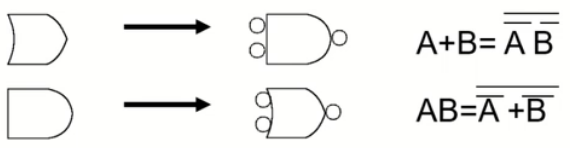
\includegraphics[width=0.6\textwidth,height=\textheight,keepaspectratio]{Krets_DeMorgan}
\end{center}

Hvis vi starter med komplementet gir dette oss følgende
\[\kom{x}\kom{y} = \overline{\var{x}+\var{y}}\]
\[\kom{x} + \kom{y} = \overline{\var{x}\var{y}}\]
Vi kan også gjøre flere i slengen:
\[\overline{\var{x} + \var{y} + \var{z}} = \kom{x}\kom{y}\kom{z}\]


\subsection{Forenkling av uttrykk}
Vi ser på representasjonformer og måter å forenkle boolske uttrykk i
seksjon~\ref{sec:bool_func} om boolske funksjoner.

\section{Logiske porter}\label{sec:logiske_porter}
Med CMOS (Seksjon~\ref{sec:cmos}) kan man lage porter som utfører logiske
operasjoner. Se figur~\ref{fig:porter}.

\begin{figure}[H]
  \centering
  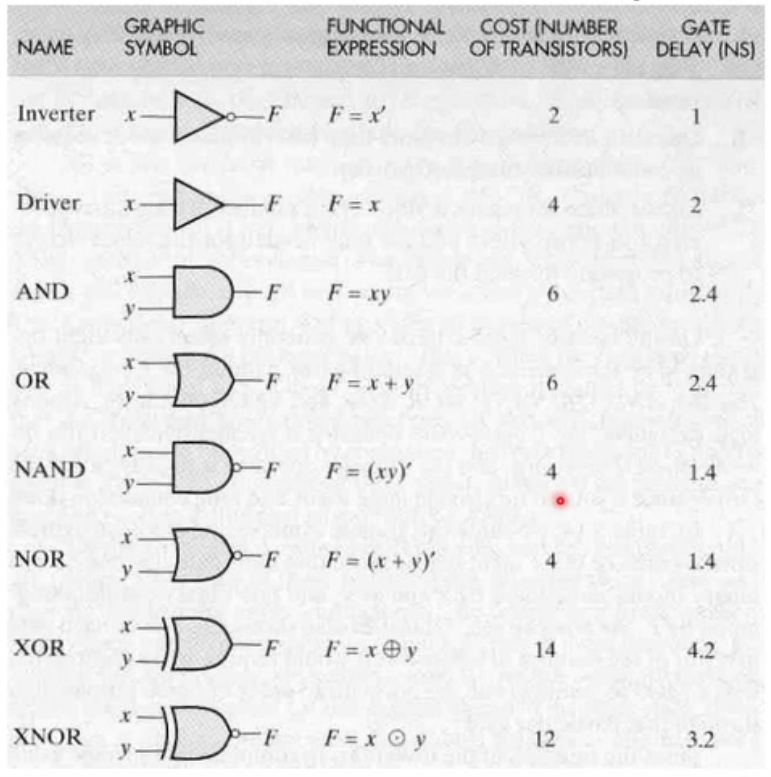
\includegraphics[width=\textwidth,height=\textheight,keepaspectratio]{Krets_Gates}
  \caption{Logiske porter, Figur 3.14 i Gajski\label{fig:porter}}
\end{figure}

\section{Forsinkelser}\label{sec:forsinkelser}
Komponenter har alltid en viss kapasitans som gjør at spenningsendriger ikke kan
skje momentant. Derfor må vi ta hensyn til forsinkelser, også i digitale
kretser, der signaler til tider vil befinne seg ``mellom'' $0$ og $1$. Vi
opererer med flere typer forsinkelser. For å finne verdiene for et gitt
komponent må vi se på komponentets datablad. Se seksjon~\ref{sec:datablader}.

\subsection{Eksempel med CMOS-inverter}
TODO\@: Sett inn eksempelet med CMOS-inverter og kondensatorer.

\begin{figure}[ht]
  \centering
  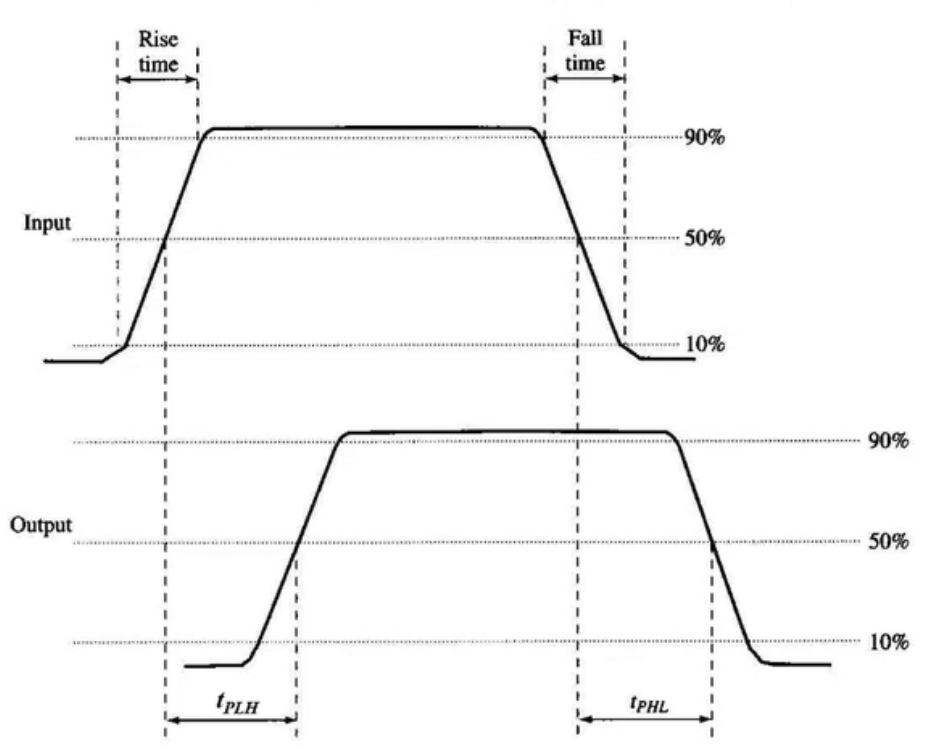
\includegraphics[width=0.8\textwidth,height=0.8\textheight,keepaspectratio]{Krets_Delay}
  \caption{Tider målt på en enkel port med input og output\label{fig:delay}}
\end{figure}

\subsection{Forplantningstid}
Forplantningstid (Propagation delay) er tiden det tar fra input har
endret seg, til output endrer seg. Oftest ser man på tiden det tar fra input har
passert $50\%$ til output passerer $50\%$. Man deler
forplantningstiden inn i $t_{PLH}$ (Output går lav til høy) og $t_{PHL}$ (Output
går høy til lav). Se figur~\ref{fig:delay}. Vi skiller mellom $t_{PHL}$ og
$t_{PLH}$ siden de kan være forskjellige, men vi har også
$t_{P} = \frac{t_{PHL}+t_{PLH}}{2}$ som vi bare kaller ``forsinkelse gjennom porten''.

Forplantningstid måles gjerne i nanosekunder. En kobberledning har en typisk
forplantningstid rundt $\frac{1}{15}$\si[per-mode =
fraction]{\nano\second\per\centi\meter}. En enkeltsående IC-chip med XOR ved
$V_{DD}=\SI{5}{\volt}$ kan ha $t_{PLH} = \SI{140}{\nano\second}$. Merk
at porter i logiske kretser oppererer rundt 1--4\si{\nano\second}. Se
seksjon~\ref{sec:logiske_porter}.

\subsection{Stigetid}
Stigetid (Rise time) er hvor lang tid det tar fra signalet
er gått fra gyldig low-verdi til gyldig high-verdi. Verdien benevnes med
$t_{TLH}$. I forelesning har vi opperert med at $10\%$ er terskelen for lav, og
$90\%$ er terskelen for høy. Se figur~\ref{fig:delay}.

\subsection{Falltid}
Falltid (Fall time) er hvor land tid det motsatte tar, altså høy til lav.
Benevnes $t_{THL}$. Se figur~\ref{fig:delay}.

\begin{figure}[h]
  \centering
  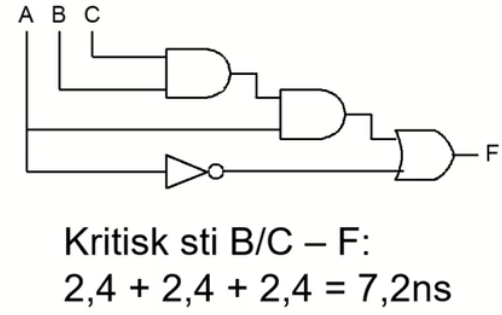
\includegraphics[width=0.6\textwidth,height=\textheight,keepaspectratio]{Krets_DuringTeknomap}
  \caption{Regning på kritisk sti i enkel logisk krets\label{fig:kritisk_sti}}
\end{figure}

\subsection{Kritisk sti}\label{sec:kritisk_sti}
Når vi skal finne forplantningstid i en krets sammensatt av flere komponenter,
må vi først finne en kritisk sti, og to input-states som, når de vekles mellom,
forursaker at et signal må propageres gjennom hele den kritiske stien før output
endrer seg. Stien er valgt slik at tiden det tar før signalet når output er størst
mulig. For å finne propageringstiden til den kritiske stien kan vi måle input og
output, og ta tiden fra input endres til output endres. Husk at
propageringstid måles fra signalet passerer $50\%$ på input til det passerer
$50\%$ av sluttoutput. Ofte vil å endre kun én input-bit gi kritisk sti, så
fremt de andre er satt riktig.

For logiske kretser med porter har vi fått oppgitt en tabell med \textit{gate
  delay} for hver port. Se seksjon~\ref{sec:logiske_porter}. Da slipper vi å
forholde oss til $t_{PLH}$ og $t_{PHL}$, og kan bare addere sammen
forsinkelsene på den tregeste veien fra en input til en output. Se
figur~\ref{fig:kritisk_sti}. Gjennom boolsk algebra er det kanskje
mulig å forbedre tiden til kritisk sti. Se seksjon~\ref{sec:tekonologimapping}
om Teknologimapping.

Husk at vi når vi bruker faktiske chipper gjerne opererer
både med $Typ$, $Min$ og $Max$-verdier for propageringstid. Total
propageringstid er altså ikke nødvendigvis worst-case, men kan være typisk
propageringstid for akkurat den input-endringen som gir propagering gjennom
den kritiske stien. En slags ``typisk for worst-case'', om du vil. Merk også at
forplantingstid, stigetid og falltid ofte er avhengige av $C_{L}$, altså
kapasitansen i output-komponentet. Lavere $C_{L}$ gir lineært raskere $t_{XXX}$.

\section{Binærtall}
TODO\@: Bruke 2-tallssystemet.

\subsection{Graykoding}
Graykoding, også kjent som ``reflected binary'', er en koding av tall der alle
nabotall har nøyaktig én bit forskjell. Man kan omdanne binærtall til og fra
Graykoding. Huskeregel: $G = B \xor (B >> 1)$.
\begin{figure}[H]
  \centering
  \begin{subfigure}{.4\textwidth}
    \centering
    \begin{align*}
      G_{7} &= B_{7} \\
      G_{6} &= B_{7} \xor B_{6} \\
            &\vdots \\
      G_{0} &= B_{1} \xor B_{0} \\
    \end{align*}
    \caption{Graykoding fra binær}
  \end{subfigure}
  \begin{subfigure}{.4\textwidth}
    \centering
    \begin{align*}
      B_{7} &= G_{7} \\
      B_{6} &= B_{7} \xor G_{6} \\
            &\vdots \\
      B_{0} &= B_{1} \xor G_{0} \\
    \end{align*}
    \caption{Binær fra graykoding}
  \end{subfigure}
  \caption{Omgjøring av 8-bit til og fra graykoding}
\end{figure}

\section{Toerkompliment}
TODO\@: Toerkompliment

\section{Regning med binærtall}
TODO\@: Sum, multiplikasjon og divisjon (med toerkompliment)

\section{Boolske funksjoner}\label{sec:bool_func}
Denne seksjonen inneholder måter å representere boolske funksjoner på, og
algebra for å forenkle boolske uttrykk med flere variabler. Husk De Morgans
teoremer og slikt fra seksjon~\ref{sec:bool_alg}.

\subsection{Kanoniske former}
Et boolsk uttrykk på kanonisk form består av OR av ANDer, eller som AND av ORer.
Alle variabler må forekomme i hvert ``ledd'', enten som ikke-komplementær eller
komplementær. Eksempel:
\[\kom{x}\kom{y} + \var{x}\var{y}\var{z} \Rightarrow \kom{x}\kom{y}\var{z} + \kom{x}\kom{y}\kom{z} + \var{x}\var{y}\var{z}\]
Vi har da gjort uttrykket om til OR av ledd der hvert ledd er ANDet og
inneholder alle variabler. Vi kaller dette oppsettet SOP, \textit{Sum of Products}.

\subsubsection{Minterm}
AND av alle variabler på enten komplementær eller ikke-komplementær form.
Indeksen til mintermen forteller hvilke variabler som er på ikke-komplementær
form. MSB av indeks svarer til første variabel, og LSB til siste. Hvis bit-en er
$0$ blir variablen på komplementær form. Se tabell~\ref{table:minterm}.

\begin{table}[H]
  \centering
  \begin{tabular}{| C | C | C |}
    \toprule
\text{Minterm} & \text{Indeks} & \text{Uttrykk} \\
    \midrule
    m_{0} & 000_{(2)} & \kom{x} \kom{y} \kom{z} \\
    m_{1} & 001_{(2)} & \kom{x} \kom{y} \var{z} \\
    m_{2} & 010_{(2)} & \kom{x} \var{y} \kom{z} \\
    \vdots & \vdots & \vdots \\
    m_{7} & 111_{(2)} & \var{x} \var{y} \var{z} \\
    \bottomrule
  \end{tabular}
  \caption{Eksempel med tre variabler $x$, $y$ og $z$\label{table:minterm}}
\end{table}

\noindent
Vi kan da omdanne en sannehetstabell til kanonisk form ved å se på hvilke rader
som gir 1, og ORe sammen mintermene til de radene. Hvis ingen av mintermene er
perfekt tilfredsstilt, blir ingen ledd 1, og uttrykket blir 0. Mintermen $m_{6}$
er altså tilfredsstilt hvis og bare hvis $(x,y,z)=(1,1,0)$.

\begin{table}[H]
  \centering
  \begin{tabular}{|c|C|C|C|C|}
    \toprule
    indeks & x & y & z & F(x,y,z) \\
    \midrule
    0 & 0 & 0 & 0 & 1 \\
    1 & 0 & 0 & 1 & 1 \\
    2 & 0 & 1 & 0 & 0 \\
    3 & 0 & 1 & 1 & 0 \\
    4 & 1 & 0 & 0 & 0 \\
    5 & 1 & 0 & 1 & 1 \\
    6 & 1 & 1 & 0 & 0 \\
    7 & 1 & 1 & 1 & 1 \\
    \bottomrule
  \end{tabular}
  \caption{Sannhetstabell for F(x,y,z)}
\end{table}

\noindent
Vi kan nå skrive F som summen av mintermene som representerer radene der $F=1$
\[F = \kom{x}\kom{y}\kom{z} + \kom{x}\kom{y}\var{z} + \var{x}\kom{y}\var{z} + \var{x}\var{y}\var{z} = m_{0}+m_{1}+m_{5}+m_{7} = \Sigma(0,1,5,7)\]
$\Sigma$ betyr altså OR av mintermene med gitt indeks.

\subsubsection{Maxterm}
OR av alle variabler på enten ikke-komplementær eller komplementær form.
\begin{center}
\begin{tabular}{ C C C }
  M_{0} & 000_{(2)} & \var{x} + \var{y} + \var{z} \\
  M_{1} & 001_{(2)} & \var{x} + \var{y} + \kom{z} \\
  M_{2} & 010_{(2)} & \var{x} + \kom{y} + \var{z} \\
  \vdots & \vdots & \vdots \\
  M_{7} & 111_{(2)} & \kom{x} + \kom{y} + \kom{z}
\end{tabular}
\end{center}
Vi kan da omdanne en sannehetstabell til kanonisk form ved å se på hvilke rader
som gir 0, og ANDe sammen maxtermene for de radene. For at en maxterm skal være
0 må den passe med raden på en prikk. Hvis noen av radene passer,
blir produktet av makstermene 0, ellers 1.

\[F = (\var{x}+\kom{y}+\var{z})(\kom{x}+\var{y}+\kom{z})(\kom{x}+\kom{y}+\var{z}) = \Pi(2,5,6)\]
$\Pi$ betyr altså AND av maxtermene med gitt indeks.

\subsubsection{Regler}
Mintermen $m_{3} = \kom{x}\var{y}\var{z}$ er kun $1$ når $(x,y,z) = (0,1,1)$ \\
Maxtermen $M_{3} = \var{x}+\kom{y}+\kom{z}$ er kun $0$ når $(x,y,z) = (0,1,1)$
%
Min tar laveste tall, er detfor AND\@. Minterm er derfor kun $1$ under riktig
omstendighet. Max tar høyeste tall, er derfor OR\@. Maxterm derfor kun $0$ under
riktig omstendighet.

\textbf{Algebra med $\Sigma$ og $\Pi$}\\
For en funksjon $F(x,y,z)$ (8 forskjellige mintermer og maxtermer)
\begin{align*}
  \Sigma(1,3,5) &= \overline{\Sigma(0,2,4,6,7)} \\
           &= \Pi(0,2,4,6,7) \\
           &= \overline{\Pi(1,3,5)}
\end{align*}

For eksempel på bruk av minterm, se seksjon~\ref{sec:fulladder} om å lage
funskoner og krets for fulladderer.

\subsection{Standardform}
Standardform er ikke like streng som kanonisk form, og vi trenger ikke nevne alle
variabler i hvert ledd. Vi må likevel forholde oss til sum av produkt (SOP)
eller produkt av sum (POS).
%
\[F_{1} = \var{x}\var{y} + \var{x}\kom{y}\var{z} + \kom{x}\var{y}\var{z}\]
%
Hvert produkt her kalles en implikant.

\subsubsection{Literalreduksjon}
Vi kan redusere antall literaler ved å gjøre algebra.
\begin{align*}
  F_{1} &= \var{x}\var{y} + \var{x}\kom{y}\var{z} + \kom{x}\var{y}\var{z} \\
        &= \var{x}\var{y}\var{z} + \var{x}\var{y}\kom{z} + \var{x}\kom{y}\var{z} + \kom{x}\var{y}\var{z} \\
        &= \var{x}\var{y}\var{z} + \var{x}\var{y}\kom{z} + \var{x}\var{y}\var{z} + \var{x}\kom{y}\var{z} + \var{x}\var{y}\var{z} + \kom{x}\var{y}\var{z} \\
        &= \var{x}\var{y}(\var{z} + \kom{z}) + \var{x}(\var{y} + \kom{y})\var{z} + (\var{x} + \kom{x})\var{y}\var{z} \\
        &= \var{x}\var{y} + \var{x}\var{z} + \var{y}\var{z}
\end{align*}
Vi har nå redusert antall literaler ned til en enklere SOP, men den kan
reduseres ytterligere.
\[\var{x}\var{y} + \var{x}\var{z} + \var{y}\var{z} = \var{x}(\var{y} + \var{z}) + \var{y}\var{z}\]
Dette er derimot ikke lenger en SOP, men en Sum av Produkt av Sum. Det er derfor
ingen grunn til å tro at kretsen blir noe raskere (snarere tvert imot), selv om
man har redusert antall literaler.

\subsection{Karnaughdiagram}
TODO\@:Skriv

\subsection{Tabellmetoden (Quine-McCluskey)}
TODO\@:Skriv. Her er engelsk Wikipedia egentlig veldig god.

\subsubsection{Elementære primledd}
Dette er ledd som garantert burde være med i SOP av utrykket.

\section{Datablader}\label{sec:datablader}
Datablader forteller oss egenskapene til komponenter når de skal brukes i kretser.
Tallene i databladene forutsetter visse omstendigheter, gjerne definert i toppen
av tabellen. Dette kan være temperatur $T_{A}$, lastkapasitans $C_{L}$ og gitt
resistiv last $R_{L}$. Databladene forutsetter også at innsignaler innfrir noen
oppgitte krav til stigetid og falltid ($t_{TLH}$, $t_{THL}$), og at spenninger
er innenfor tilatte skranker.

\subsection{Oppgitte verdier}
\textbf{Forplantingstid}, \textbf{Stigetid}, og \textbf{Falltid}\\
Disse forsinkelsene kalles henholdsvis $t_{PLH}$/$t_{PHL}$, $t_{TLH}$ og
$t_{THL}$. Se seksjon~\ref{sec:forsinkelser} om forsinkelser.

\textbf{Inputkapasitans}\\
Input har en viss kapasitans $C_{in}$, altså må en viss mengde strøm tilføres for å endre
spenningen opp til høy, eller motsatt for høy til lav.

\textbf{Gyldige spenninger}\\
$V_{DD}$ er driftspenningen, og andre egenskaper påvirkes av driftsspenningen.
$V_{IL}$ er hvilken skranke en input-spenning må ligge i for å anerkjennes som
lav. $V_{IH}$ er skranken for høy input-spenning.

\section{Logiske kretser}\label{sec:logic_circuits}
Nå skal vi bruke det vi vet om sannhetstabeller, algebra, porter og forsinkelse
til å lage kretser som utfører boolske funskjoner raskt og med få transistorer.

\subsection{1-bit fulladder}
TODO:\ Skriv.

\subsection{Ripple-carry fulladder}\label{sec:ripple_carry_fulladder}
Én måte å addere sammen to $n$-bits tall er å bruke $n$ 1-bits full-addere, med
carry propagert fra LSB oppover til MSB\@. Svaret blir et $n$-bits tall med
carry. Dette ligner måten addisjon gjøres for hånd. Problemet med denne adderen
er at carry må propageres helt fra LSB til MSB, og kritisk sti blir veldig lang.
(Hint: $0b01111111 + 1$)

\subsection{Carry-lookahead adder}
TODO:\ Skriv

\section{Teknologimapping}\label{sec:tekonologimapping}
Målet er å konvertere en logisk krets slik at den benytter kun tilgjengelige
porter, f.eks.\ kun NAND eller kun NOR\@. Vi
ønsker også å redusere lengden på kritisk sti (Se seksjon~\ref{sec:kritisk_sti}), og
redusere totale antall transistorer (Se seksjon~\ref{sec:logiske_porter}). Måten vi
gjør det på er ved å dekomponere innganger (3-inputs AND $\Rightarrow$ 2 stykk 2-inputs
AND), og konvertere porter med boolalgebraiske identiteter. Eksempler:
\begin{align*}
  \var{x}\var{y} &= \overline{\overline{\var{x}\var{y}}} & \text{AND = NOT
                                                           NAND} \\
  \var{x}+\var{y} &= \overline{\overline{\var{x}+\var{y}}} & \text{OR = NOT
                                                           NOR} \\
  \var{x}+\var{y} &= \overline{\kom{x}\kom{y}} & \text{OR = NAND av NOT} \\
  \var{x}\var{y} &= \overline{\kom{x}+\kom{y}} & \text{AND = NOR av NOT} \\
  \overline{\kom{x}} &= \var{x} & \text{NOT NOT kanselleres}
\end{align*}

Dette er litt tricky, så jeg tar med to eksempler.

\subsection{Eksempel med NAND og NOT}
Vi skal konvertere følgende krets til å bare bruke NAND og INV (Inverter = Not).
\begin{center}
  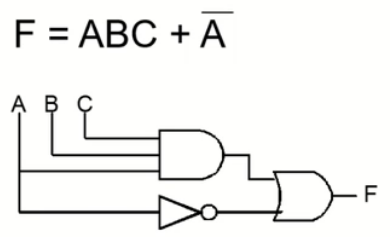
\includegraphics[width=0.6\textwidth,height=\textheight,keepaspectratio]{Krets_BeforeTeknomap}
\end{center}
Det første vi gjør er å bytte AND-3 til 2 stykk AND-2 i serie.
\begin{center}
  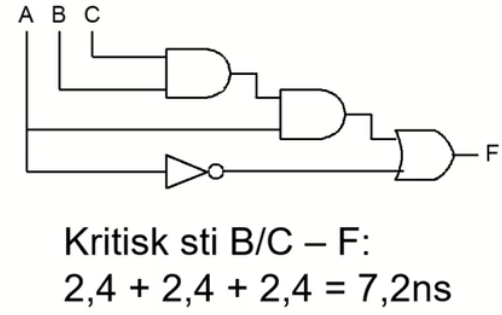
\includegraphics[width=0.6\textwidth,height=\textheight,keepaspectratio]{Krets_DuringTeknomap}
\end{center}
Dette gir en krets som vi lett kan lage med komponenter, men den kritiske stien blir
\SI{7.2}{\nano\second}. Vi kan gjøre om AND om til NOT NAND, og ved å bruke De
Morgan får vi gjort OR om til NAND av NOTs. Vi fjerner dobbel invertering, og
ender opp med kretsen under.
\begin{center}
  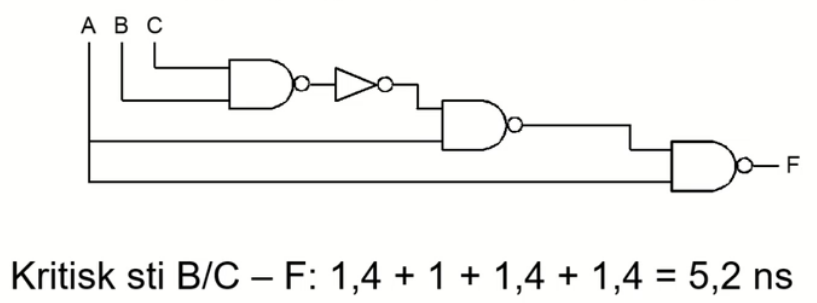
\includegraphics[width=0.6\textwidth,height=\textheight,keepaspectratio]{Krets_AfterTeknomap}
\end{center}
Vi har nå den samme kretsen, men med kun NAND og NOT, slik oppgaven ba om. Her
blir altså den kritiske stien kortere, selv om det er flere komponenter. Dette
skyldes i stor grad at NAND er rask. Dessuten bruker NAND kun 4 transistorer.

\subsubsection{Input-delay}
Dersom vi vet at en av inputene kommer fra en annen krets med en ekstra forsinkelse,
kan vi legge opp kretsen vår på en annen måte, for å minimere total kritisk sti. La oss si
at input C er forsinket med $X$\si{\nano\second}.
\begin{center}
  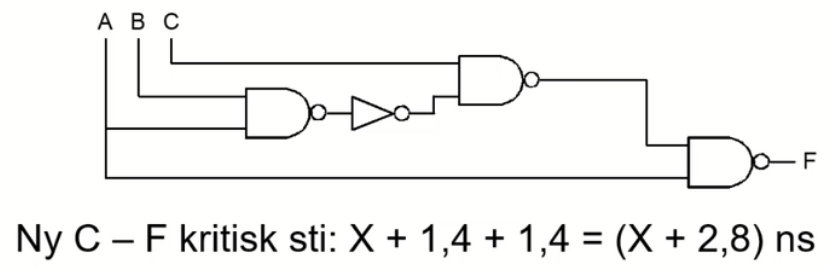
\includegraphics[width=0.6\textwidth,height=\textheight,keepaspectratio]{Krets_CTeknomap}
\end{center}
Her er det teknisk sett \@A/B\@--\@F som er kritisk sti, men siden vi tar hensyn til
$X$, minimerer vi heller det som legges til $X$, altså \@C\@--\@F\@.

\subsection{Eksempel med kun NOR}
Vi ønsker å lage en logisk krets for den boolske funksjonen
\[T = BD + \bar{A}B\bar{C} + \bar{A}CD\]
TODO

\section{PAL}
TODO

\section{Sekvensielle kretser}
Tidligere har vi forholdt oss til kombinatoriske kretser, der et sett med input
passerer gjennom én eller flere boolske funksjoner og blir output. En sekvensiell
krets har tilstand, som betyr at input til kretsen ikke bare kommer utenfra, men
også fra inni kretsen selv. Sannhetstabeller inneholder derfor nåværende tilstand
som input, og neste tilstand som output. Hvis man ikke er forsiktig kan dette gi
ustabile løkker, f.eks.\ en inverter som mater inn i seg selv og flyter mellom 0
og 1.

\begin{center}
  \fbox{\begin{minipage}{.8\textwidth}
      \addtocontents{toc}{Låser vs. vipper}
    \textbf{Låser vs. vipper}\\
    Det later til å være variasjon i navnsetting av komponentene som følger. I
    dette dokumentet har jeg valgt å bruke \textit{lås} om alt som er
    nivåstyrt (eller ikke har noe styring), og \textit{vippe} om det som
    er flankestyrt. Dette er basert på diverse engelske definisjoner av
    henholdsvis \textit{latch} og \textit{flip-flop}.
  \end{minipage}}
\end{center}

\subsection{SR-lås}
En SR-lås er en sekvensiell krets bestående av to NOR-porter koblet i ``kryss''.
I tillegg kommer input $S$ og $R$ som står for \textit{Set} og \textit{Reset}.
Hver NOR-port har output ut av kretsen i tillegg til inn igjen i motsatt NOR\@.
Disse blir SR-låsens outputs, $Q$ og $\bar{Q}$. Se Figur~\ref{fig:SR-latch}.

\begin{figure}[hbt!]
  \centering
  \begin{minipage}{0.5\textwidth}
    \centering
    \begin{circuitikz} \draw
      (3,3) node[american nor port](R_NOR){}
      (3,0) node[american nor port](S_NOR){}

      (S_NOR.in 2) -- ++(-1,0) node[left]{$S$}
      (R_NOR.in 1) -- ++(-1,0) node[left]{$R$}

      (S_NOR.in 1) -- ++(-1,0) node[inner sep=0](S_IN){}
      (R_NOR.in 2) -- ++(-1,0) node[inner sep=0](R_IN){}

      (R_NOR.out) to[short,-*] ++(.5,0) node[inner sep=0](R_OUT){} -- ++(0,-.5) -- (S_IN)
      (S_NOR.out) to[short,-*] ++(.5,0) node[inner sep=0](S_OUT){} -- ++(0,.5)  -- (R_IN)

      (R_OUT) -- ++(1,0) node[right]{$Q$}
      (S_OUT) -- ++(1,0) node[right]{$\bar{Q}$}
      ;
    \end{circuitikz}
    \caption{Portdiagram for SR-lås \label{fig:SR-latch}}
  \end{minipage}\hfill
  \begin{minipage}{.45\textwidth}
    \centering
    \begin{tabular}{cc|cc}
      \toprule
      S & R & Q & $\bar{\text{Q}}$ \\
      \midrule
      0 & 0 & \multicolumn{2}{c}{Uendret} \\
      0 & 1 & 0 & 1 \\
      1 & 0 & 1 & 0 \\
      1 & 1 & \red{0} & \red{0} \\
      \bottomrule
    \end{tabular}
    \captionof{table}{Sannhetstabell for SR-lås\label{tab:SR-latch}}
  \end{minipage}
\end{figure}

SR-låsen fungerer ved at én av NOR-portene gir høy output, som får den andre til å
ha lav output. $Q$ og $\bar{Q}$ er altså motsatte under vanlig drift. Med $S$ og $R$
kan man styre hvilke NOR-porter som gjør hva. Når $S$ blir satt høy vil
NOR-porten til $\bar{Q}$ bli lav, som setter NOR-porten til $Q$ høy, som igjen går
inn i $\bar{Q}$ sin NOR-port og holder den lav. Motsatte skjer for $R$. Resultatet er
at en høy input på \textit{Set} setter $Q$ høy helt til \textit{Reset} blir satt
høy, som resetter $Q$ til lav. Se Tabell~\ref{tab:SR-latch}.

Før $S$ eller $R$ har vært høye er det umulig å vite tilstanden til bryteren.
Dersom både $S$ og $R$ er høye samtidig blir både $Q$ og $\bar{Q}$ $0$, og hvis begge
inputs går lave samtidig blir tilstanden igjen ubestemt.

\subsection{Eksitasjonstabell}
En eksitasjonstabell viser hvilke inputs som forursaker en ønsket
tilstandforandring. Venstresiden har nåværende og ønsket tilstand, og høyresiden
har hva input må være. Dersom en av inputenes tilstand ikke er vesentlig brukes $X$. For
et eksempel med SR-lås, se Tabell~\ref{tab:SR_latch_eksit}.

\begin{table}[hbt!]
  \centering
  \begin{tabular}{cc|cc}
    \toprule
    Q & Q$_{next}$ & S & R \\
    \midrule
    0 & 0 & 0 & X \\
    0 & 1 & 1 & 0 \\
    1 & 0 & 0 & 1 \\
    1 & 1 & X & 0
  \end{tabular}
  \caption{Eksitasjonstabell for SR-lås\label{tab:SR_latch_eksit}}
\end{table}

\subsection{Styrt SR-lås}
En styrt SR-lås er en SR-lås der $S$ og $R$ kun har en virkning når en tredje
input $EN$ er høy. Dette ser man i blant annet en D-lås.

\subsection{D-lås}
En D-lås er en styrt SR-lås med kun én data-inngang $D$ og enable-inngangen
$EN$. SR-låsens input $S$ kommer fra $D$, og $R$ kommer
fra $\bar{D}$. Se Figur~\ref{fig:D-latch}.

\begin{figure}[hbt!]
  \centering
  \begin{circuitikz} \draw
    (3,3) node[american nor port](R_NOR){}
    (3,0) node[american nor port](S_NOR){}

    (S_NOR.in 2) -- ++(-1,0) node[american and port](S_AND){}
    (R_NOR.in 1) -- ++(-1,0) node[american and port](R_AND){}

    (S_NOR.in 1) -- ++(-1,0) node[inner sep=0](S_IN){}
    (R_NOR.in 2) -- ++(-1,0) node[inner sep=0](R_IN){}

    (R_NOR.out) to[short,-*] ++(.5,0) node[inner sep=0](R_OUT){} -- ++(0,-.5) -- (S_IN)
    (S_NOR.out) to[short,-*] ++(.5,0) node[inner sep=0](S_OUT){} -- ++(0,.5)  -- (R_IN)

    (R_OUT) -- ++(1,0) node[right]{$Q$}
    (S_OUT) -- ++(1,0) node[right]{$\bar{Q}$}

    (S_AND.in 1) -- ++(-.3,0) node[inner sep=0](S_EN){}
    (R_AND.in 2) -- ++(-.3,0) -- (S_EN) node[midway,inner sep=0](EN){}
    (EN) -- ++(-.8,0) node[left]{EN}

    (R_AND.in 1) node[above]{R} ++(-1,0) node[american not port](NOT){}
    (R_AND.in 1) ++(-2,0) coordinate(R_NOT_IN)
    (R_AND.in 1) -- (NOT.out)

    (S_AND.in 2) node[below]{S} -- ++(-2,0) node[circ](D){} -- (R_NOT_IN) -- (NOT.in)
    (D) -- ++(-1,0) node[left]{$D$}
    ;
  \end{circuitikz}
  \caption{Portdiagram for D-lås \label{fig:D-latch}}
\end{figure}

Når $EN$ er høy vil enten $S$ eller $R$ være høy, og SET/RESET-tilstanden blir
lagret. Når $EN$ blir lav vil tilstanden holdes, uavhengig av $D$.
En D-lås kan ses på som én bit med hukommelse, som husker hva $D$ var sist gang
$EN$ var høy. Se Tabell~\ref{tab:D-latch}.

\newcommand{\ubercol}[1]{\begin{tabular}{@{}c@{}}#1\end{tabular}}

\begin{table}[hbt!]
  \centering
  \begin{minipage}{.45\textwidth}
    \centering
    \begin{tabular}{ccc|c}
      \toprule
      D & EN & Q & Q$_{next}$\\
      \midrule
      X & 0 & 0 & 0 \\
      X & 0 & 1 & 1 \\
      1 & 1 & X & 1 \\
      0 & 1 & X & 0 \\
      \bottomrule
    \end{tabular}
    \caption{Sannhetstabell for D-lås\label{tab:D-latch}}
  \end{minipage}\hfill
  \begin{minipage}{.45\textwidth}
    \centering
    \begin{tabular}{cc|cc}
      \toprule
      Q & Q$_{next}$ & D & EN\\
      \midrule
      0 & 0 & \ubercol{X\\0} & \ubercol{0\\X} \\
      \midrule
      0 & 1 & 1 & 1 \\
      \midrule
      1 & 0 & 0 & 1 \\
      \midrule
      1 & 1 & \ubercol{X\\1} & \ubercol{0\\X} \\
      \bottomrule
    \end{tabular}
    \captionof{table}{Eksitasjonstabell for D-lås\label{tab:D-latch-eksit}}
  \end{minipage}
\end{table}

\section{Tidsdiagrammer}
TODO

\section{Klokkestyring}
Vi instroduserer et klokkesignal i kretsen for å kunne synkronisere dataflyt
mellom flere komponenter. Som oftest ser klokkesignalet ut som en firkantpuls
med 50\% høyt og 50\% lavt signal. Øyeblikket lav går til høy kalles stigende
flanke, og motsatt kalles synkedne flanke. Frekvensen blir antall stigende
flanker per sekund.

\subsection{Klokkestyrt D-lås}
En D-lås er allerede styrt med $EN$-inputen. For å gjøre den klokkestyrt kobler
man klokken til $EN$. Dette blir da en nivåstyrt lås, som henter inn data når
klokken er høy, og holder på dataen når klokken er lav.

\subsection{Oppsett- og holdetid}
$t_{setup}$ er tiden datasignalet må være stabilt før en endring i
klokkesignalet kan skje. $t_{hold}$ er tiden datasignalet må være stabilt etter
en endring i klokkesignal. Dette er fordi forsinkelser i porter gjør at
signalforandringer bruker en viss tid på å propagere ferdig. Hvis et annet
signal endres undeveis vil propageringen kunne skje kun delvis, og sluttilstanden
blir udefinert. For nivåstyrte kretser gjelder $t_{hold}$ fra nivået slutter.
For flankestyrte kretser er $t_{hold}$ tiden man må holde etter trigger-flanken.

\section{Flankestyring}
Forrige seksjon brukte klokkesignalet for å bestemme når data kunne endres, og
når data var låst fast. Dette kalles nivåstyring, siden nivåene på
klokkesignalet har betydning. I denne seksjonen er det ikke nivået som er
viktig, men øyeblikket nivået endres. Når klokke går fra lav til høy kaller vi
det stigende klokkeflanke (\rising), og motsatt høy til lav kalles synkende
klokkeflanke (\falling).
Vi opererer gjerne med at endringen skjer momentant, og at klokken er en perfekt
firkantbølge. Et flankestyrt komponent bryr seg ofte kun om én av flankene.

\subsection{Triggring}
Når et flankestyrt komponent mottar riktig flanke kaller vi det triggring. Da
hentes data inn fra input, og behandles av kretsen. Verdien på input er kun interresant i
trigger-øyeblikket, og frem til neste triggring vil kretsen være helt likegyldig
til input. Så lenge input er stabil i $t_{setup}$ før trigging, og $t_{hold}$
etter, kan input være hva enn den bare vil resten av tiden og ikke ha
noe å si.

I blokkdiagrammer har man et symbol for å vise at triggring skjer på stigende
klokkeflanke, se Figur~\ref{fig:SR-flip-flop-block}. Hvis triggring skjer på synkende
flanke vil klokkeinputen ha en sirkel foran seg, likt en pMOS\@.

\subsection{SR-vippe}
Aller først gjør vi en SR-lås til en SR-vippe, bare for å vise blokkdiagramformen,
sannhetstabellen, og timingdiagrammet. Se Figur~\ref{fig:SR-flip-flop-block} og Tabell~\ref{tab:}.

\begin{figure}[hbt!]
  \centering
  \begin{minipage}{.45\textwidth}
    \centering
    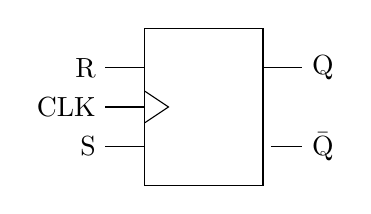
\begin{tikzpicture}
      \draw (0,0) rectangle (1.5,2);
      \draw (0,.8) -- (.3,1) -- (0,1.2);
      \draw (0,1) -- ++(-.5,0) node[left]{CLK};
      \draw (0,0.5) -- ++(-.5,0) node[left]{S};
      \draw (0,1.5) -- ++(-.5,0) node[left]{R};
      \draw (1.5,1.5) -- ++(.5,0) node[right]{Q};
      \draw (1.5,0.5) circle ++(.1,0) -- ++(.4,0) node[right]{$\bar{\text{Q}}$};
    \end{tikzpicture}
    \caption{Blokkdiagramform av SR-vippe\label{fig:SR-flip-flop-block}}
  \end{minipage}\hfill
  \begin{minipage}{.45\textwidth}
    \centering
    \begin{tabular}{ccc|cc}
      \toprule
      S & R & CLK & Q & $\bar{\text{Q}}$ \\
      \midrule
      0 & 0 & \rising{} & \multicolumn{2}{c}{Uendret} \\
      1 & 0 & \rising{} & 1 & 0 \\
      0 & 1 & \rising{} & 0 & 1 \\
      1 & 1 & \rising{} & \red{0} & \red{0} \\
      X & X & X & \multicolumn{2}{c}{Uendret} \\
      \bottomrule
    \end{tabular}
    \captionof{table}{\label{tab:}}
  \end{minipage}
\end{figure}

\subsection{D-vippe (Master-slave-vippe)}
To D-vipper i serie, der den éne mater den andre, men med omvendt klokkesignal. Se
figur~\ref{fig:master_slave}. Dette gjøres slik at å lese input $D$ og sende
output $Q$ er uavhengige. I vårt eksempel vil $D$ leses inn så lenge
klokken er lav, og i øyeblikket klokken går høy ``trigger'' vi vippen, og
signalet sendes ut $Q$. Endringer på $D$ vil ikke påvirke $Q$ før
neste triggring.

\begin{figure}[hbt!]
  \centering
  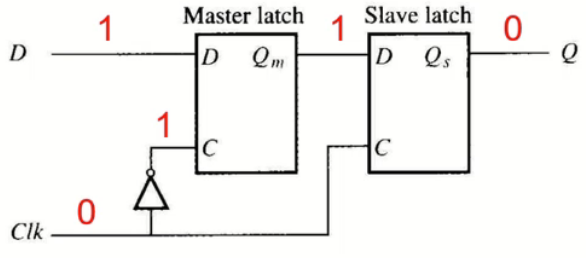
\includegraphics[width=0.7\textwidth,height=\textheight,keepaspectratio]{Krets_MasterSlave}
  \caption{D-vippe - to D-låser i master-slave-oppsett\label{fig:master_slave}}
\end{figure}

\begin{table}[hbt!]
  \centering
  \begin{tabular}{cc|cc}
    \toprule
    D & CLK & Q & $\bar{\text{Q}}$ \\
    \midrule
    0 & \rising{} & 0 & 1\\
    1 & \rising{} & 1 & 0\\
    X & X & \multicolumn{2}{c}{Uendret}\\
    \bottomrule
  \end{tabular}
  \caption{Sannhetstabell for D-vippe}
\end{table}

\subsection{Shift-register}
Ved å legge flere flankestyrte D-vipper i serie kan vi lage et shift-register der
flere bits er lagret i en slags kø, og kan shiftes bortover samtidig. Se Figur~\ref{fig:trigger_shift}.

\begin{figure}[hbt!]
  \centering
  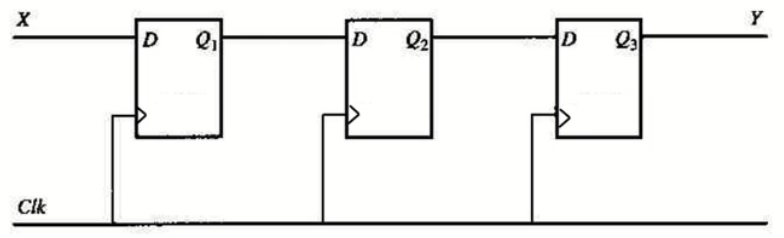
\includegraphics[width=0.7\textwidth,height=\textheight,keepaspectratio]{Krets_TriggerShift}
  \caption{Et shiftregister laget av flere master-slave-vipper i serie med samme trigger\label{fig:trigger_shift}}
\end{figure}

Hver av disse master-slave-vippene holder en verdi som de sender ut av hendholdsvis $Q_{1}$,
$Q_{2}$, $Q_{3}$. Ved stigende klokkeflanke vil hver vippe overskrives av det
den fikk inn i akkurat det øyeblikket. Resultatet er at køen går fremover.
Verdien i $Q_{3}$ forsvinner, og de andre verdiene rykker én plass frem. Verdien
$X$ stiller seg bakerst i køa.
\[
  Q_{3} \leftarrow Q_{2} \hspace{10mm} Q_{2} \leftarrow Q_{1} \hspace{10mm}  Q_{1} \leftarrow X
\]

\subsection{JK-vippe}
TODO
En JK-lås er en toggle

\subsection{T-vippe}
TODO
En T-lås er en toggle


\subsection{Registere}
TODO

\end{document}
